%!TEX encoding = UTF-8 Unicode
% ================================================================================
\documentclass[
    fontsize=12pt,
    headings=small,
    parskip=half,           % Ersetzt manuelles Setzen von parskip/parindent.
    bibliography=totoc,
    numbers=noenddot,       % Entfernt den letzten Punkt der Kapitelnummern.
    open=any,               % Kapitel kann auf jeder Seite beginnen.
%   final                   % Entfernt alle todonotes und den Entwurfstempel.
    ]{scrreprt}
% ===================================Praeambel==================================
%!TEX encoding = UTF-8 Unicode
%!TEX root = hinweiseabschlussarbeit.tex

% Kodierung, Sprache, Patches {{{
\usepackage[T1]{fontenc}    % Ausgabekodierung; ermöglicht Akzente und Umlaute
                            %  sowie korrekte Silbentrennung.
\usepackage[utf8]{inputenc} % Erlaubt die direkte Eingabe spezieller Zeichen;
                            %  utf8 muss die Eingabekodierung des Editors sein.
\usepackage[ngerman]{babel} % Deutsche Sprachanpassungen (z.B. Überschriften).
\usepackage{microtype}      % Optimale Randausrichtung und Skalierung.
\usepackage[
    autostyle,
    ]{csquotes}             % Korrekte Anführungszeichen in der Literaturliste.
%\usepackage{fixltx2e}      % Patches fuer LaTeX2e - seit 2015 nicht mehr nötig
\usepackage{scrhack}        % Verhindert Warnungen mit älteren Paketen.
\usepackage[
  newcommands
]{ragged2e}                 % Verbesserte \ragged...Befehle
\PassOptionsToPackage{
  hyphens
}{url}                      % Sorgt für URL-Umbrüche in Fußzeilen u. Literatur
% }}}

% Schriftarten {{{
\usepackage{mathptmx}       % Times; modifies the default serif and math fonts
\usepackage[scaled=.92]{helvet}% modifies the sans serif font
\usepackage{courier}        % modifies the monospace font
% }}}

% Biblatex {{{
\usepackage[
    style=alphabetic,
    backend=biber,
    %backref=true
    ]{biblatex}             % Biblatex mit alphabetischem Style und biber.
\bibliography{literaturliste.bib} % Dateiname der bib-Datei.
\DeclareFieldFormat*{title}{
    \mkbibemph{#1}}         % Make titles italics
% }}}

% Dokument- und Texteinstellungen {{{
\usepackage[
    a4paper,
    margin=2.54cm,
    marginparwidth=2.0cm,
    footskip=1.0cm
    ]{geometry}             % Ersetzt 'a4wide'.
\clubpenalty=10000          % Keine Einzelzeile am Beginn eines Absatzes
                            %  (Schusterjungen).
\widowpenalty=10000         % Keine Einzelzeile am Ende eines Absatzes
\displaywidowpenalty=10000  %  (Hurenkinder).
\usepackage{floatrow}       % Zentriert alle Floats
\usepackage{ifdraft}        % Ermöglicht \ifoptionfinal{true}{false}
\pagestyle{plain}           % keine Kopfzeilen
% \sloppy                    % großzügige Formatierungsweise
\deffootnote{1em}{1em}{
  \thefootnotemark.\ }      % Verbessert Layout mehrzeiliger Fußnoten
\ifdefined\chapterformat
	\renewcommand*{\chapterformat}{% Hübscht Kapitelüberschrift mit senkrechtem 
		\thechapter\enskip%          grauen Balken zwischen Nummer und Text auf
		\textcolor{gray!50}{\rule[-\dp\strutbox]{2pt}{\baselineskip}}\enskip
	}
\fi
%\setkomafont{disposition}{\normalcolor\bfseries} % Aus der KOMA-Skript-Anleitung: „Mit dieser Änderung verzichten Sie darauf, für alle Gliederungsebenen serifenlose Schrift voreinzustellen“

\makeatletter
\AtBeginDocument{%
    \hypersetup{%
        pdftitle = {\@title},
        pdfauthor  = \@author,
    }
}
\makeatother
% }}}

\newcommand*\rot[1]{\rotatebox{90}{#1}}

% Weitere Pakete {{{
\usepackage{graphicx}       % Einfügen von Graphiken.
\usepackage{tabu}           % Einfügen von Tabellen.
\usepackage{multirow}       % Tabellenzeilen zusammenfassen.
\usepackage{multicol}       % Tabellenspalten zusammenfassen.
\usepackage{booktabs}       % Schönere Tabellen (\toprule\midrule\bottomrule).
\usepackage[nocut]{thmbox}  % Theorembox bspw. für Angreifermodell.
\usepackage{amsmath}        % Erweiterte Handhabung mathematischer Formeln.
\usepackage{amssymb}        % Erweiterte mathematische Symbole.
\usepackage{rotating}
\usepackage{longtable}      % for 'longtable' environment
\usepackage{pdflscape}      % for 'landscape' environment
\usepackage{xltabular}
\usepackage[
    printonlyused
    ]{acronym}              % Abkürzungsverzeichnis
\usepackage[
    colorinlistoftodos,
    textsize=tiny,          % Notizen und TODOs - mit der todonotes.sty von
    \ifoptionfinal{disable}{}%  Benjamin Kellermann ist das Package "changebar"
    ]{todonotes}            %  bereits integriert.
\usepackage[
    breaklinks,
    hidelinks,
    pdfdisplaydoctitle,
    pdfpagemode = {UseOutlines},
    pdfpagelabels,
    ]{hyperref}             % Sprungmarken im PDF. Lädt das URL-Paket.
    \urlstyle{rm}           % Entfernt die Formattierung von URLs.
%\usepackage{breakurl}
%\def\UrlBreaks{\do\/\do-}
\usepackage{listings}       % Spezielle Umgebung für Quelltextformatierung.
    \lstset{                
        language=C,
        breaklines=true,
        breakatwhitespace=true,
        frame=l,            % Linie links: l, doppelt: L
		framerule=2.5pt,    % Dicke der Linie
		rulecolor=\color{gray},% Farbe der Linie
        captionpos=b,
        xleftmargin=6ex,
        tabsize=4,
        numbers=left,
        numberstyle=\ttfamily\footnotesize,
        basicstyle=\ttfamily\footnotesize,
        keywordstyle=\bfseries\color{green!50!black},
        commentstyle=\itshape\color{magenta!90!black},
        identifierstyle=\ttfamily,
        stringstyle=\color{orange!90!black},
        showstringspaces=false,
        }

\usepackage{algorithm}
\usepackage{algpseudocode}
%\usepackage{filecontents}  % Direktes Einfügen von Dateiinhalt. Wird hier für
                            %  die Verwendung einer .bib-Datei in dieser .tex-
                            %  Datei benötigt.
% }}}

% ===================================Dokument===================================

\title{Intrusion detection for OAuth}
\author{Florian Nehmer}
\date{06.01.2023} % Falls ein bestimmtes Datum eingesetzt werden soll, einfach
                    %  diese Zeile aktivieren.

\begin{document}

\begin{titlepage}% {{{
	
\includegraphics[width=6.8cm]{./pic/up-uhh-logo-u-2010-u-farbe-u-rgb.pdf}
	\begin{center}\Large
		\vfill
		Masterarbeit
		\vfill
		\makeatletter
		{\Large\textsf{\textbf{\@title}}\par}
		\makeatother
		\vfill
		vorgelegt von
		\par\bigskip
		\makeatletter
		{\@author} \par
		\makeatother
		Matrikelnummer 6417446 \par
		Studiengang Informatik
		\vfill
		MIN-Fakultät \par
		Fachbereich Informatik
		\vfill
		\makeatletter
		eingereicht am {\@date}
		\makeatother
		\vfill
		Betreuer: Pascal Wichmann, M.\,Sc. Informatik \par
		Erstgutachter: Prof. Dr.-Ing. Hannes Federrath \par
		Zweitgutachter: Pascal Wichmann, M.\,Sc. Informatik.
	\end{center}
	\ifoptionfinal{}{
	\begin{tikzpicture}[remember picture, overlay]
		\node[draw, red, font=\ttfamily\bfseries\Large, xshift=30mm, yshift=238mm,
			rotate=340, text centered, text width=6cm, very thick, rounded
			corners=4mm] at (current page.south) {Entwurf vom \today};
	\end{tikzpicture}
	% ====> Delete me
	\begin{tikzpicture}[overlay]
		\node[draw, blue, font=\sffamily\Large, xshift=0mm, yshift=210mm, rotate=0, text centered, rounded corners=1mm] at (current page.south) {Muster des Deckblatts für Abschlussarbeiten};
	\end{tikzpicture}
	% <==== /Delete me
	}
\end{titlepage}% }}}

\chapter*{Aufgabenstellung}
OAuth [RFC6749] is a widely used authentication protocol, which is typically used between multiple actors, such as different organizations. As authentication is at the core of application security, it is specifically essential to prevent attacks on the authentication.

The tasks of this thesis are as follows: Firstly, a systematic literature study should be performed on existing properties and attacks on the OAuth protocol or its implementations. Secondly, the thesis should design protection strategies for the threats that are not sufficiently solved in existing solutions. Two options for this step are (i) the utilization of anomaly-based intrusion detection for OAuth and (ii) specification-based intrusion detection for OAuth. Thirdly, the thesis should evaluate the security of the designed architecture and compare it to other solutions.

\chapter*{Zusammenfassung}

Für die eilige Leserin bzw. den eiligen Leser sollen auf etwa einer halben, maximal einer Seite die wichtigsten Inhalte, Erkenntnisse, Neuerungen bzw. Ergebnisse der Arbeit beschrieben werden.

Durch eine solche Zusammenfassung (im Engl. auch Abstract genannt) am Anfang der Arbeit wird die Arbeit deutlich aufgewertet. Hier sollte vermittelt werden, warum man die Arbeit lesen sollte.

\tableofcontents

\chapter{Introduction}
\label{chap.introduction}
\section{Motivation}
\todo{Write Motivation}
\section{Research Question}
\todo{Write down Research Question}
\section{Outline}
\todo{Decide if Outline is necessary}

\chapter{Fundamental Knowledge}
\label{chap.fundamental_knowledge}
\todo{Write Introduction to Fundamental knowledge chapter}

\section{OAuth 2.0 protocol}
The Open Authorization 2.0 protocol nowadays often referred to as the
\emph{OAuth} protocol, is an authorization framework, that allows third-party
applications to gain limited access to resources in a different location on
behalf of the party, that owns these resources. For many users of the Internet,
it is in practice the protocol behind the ``\emph{Sign in with ...}'' button.
The current standard, first defined in 2012 in RFC6749, is already the
successor of the OAuth 1.0 standard, which was officially published in 2010 by
the IETF in RFC5849 \cite{hammer2010rfc}. In the meantime, several extensions
for the protocol were published as standards and technical reports. These
extensions include new functionalities for the protocol e.g. the ability to use
the protocol with devices like smart TVs and printers \cite{denniss2019oauth}
or documents, which describe several security considerations when implementing
the protocol in practice \cite{lodderstedt2020oauth}. As a whole, the OAuth
working group of the Internet Engineering Task Force (IETF) submitted a total
of 30 Request for Comments (RFCs) and 16 active drafts, from which 7 are active
individual drafts. Table X shows a complete list of all OAuth 2.0. related IETF
submissions by the OAuth working group. 

\subsection{Involved parties}
Because the OAuth protocol is very diverse and complex, as it is a
whole authorization framework it makes sense to narrow it down to its core
features. Starting with the involved parties in the protocol. In general there
are four parties involved in the most common OAuth protocol modes:

\begin{itemize} 

    \item Resource owner: The resource owner is the entity that owns or is
        allowed to manage protected resources. The resource owner might grant
        access to these resources. 

    \item Resource server: The resource server is the server, where the
        protected resources are stored. It can accept or decline authorization
        tokens, which it receives from the client. 

    \item Client: The client is an entity, which makes requests to get access
        to the protected resources, on behalf of the resource owner. 
        
    \item Authorization server: The server, that manages access to the
        protected data. It issues access tokens to the client after successful
        authentication of the resource owner. 

\end{itemize}

Depending on the protocol mode, these four parties or in some cases three
parties exchange different messages in variable ways. In general, there are two
different types of messages, which are explained in the next section.

\subsection{Front-channel and Back-channel messages}

Regarding security considerations messages of the OAuth framework can be
categorized into two main categories, \emph{front-channel} and
\emph{back-channel}. As the protocol is mostly used in the application layer
using HTTP and TLS, \emph{front-channel} means that the message is transported
via the \emph{Request-URI} \cite[Sec. 5.1.2]{fielding1999hypertext} e.g. by
using query parameters. \emph{Back-channel} means on the other hand that the
message is transported via the HTTP message body. In other words, back-channel
messages are transported in one TCP connection, between caller and receiver,
whereas front-channel messages use redirects. \cite[p. 338]{belfaik2022single}.

\subsection{Grant Types}
The protocol flow is dependent on the protocol mode. In the case of OAuth the
different protocol modes are called \emph{Grant types}, as the modes differ on
how the authorization is granted to the resource owner via the client.

\subsubsection{Authorization Code Grant}
According to a recent study, the authorization code grant mode of OAuth is the
most used protocol mode for OAuth on the internet
\cite[Table1]{philippaerts2022oauch}. It is offered by more than 90\% of common 
identity providers.

In this mode illustrated in Figure 2.1, a resource owner aiming to access
protected data via a REST API utilizes a user agent, in this case the web
browser, to interact with a client application that executes API requests
through the user agent. The process begins as the client redirects the user
agent to the authorization server through the front channel. The message
contains a client ID, a redirect URL and a state. The client ID is a unique
identifier of the protected resource. The redirect URI is the location the user
agent is redirected to after authentication. The state can hold any string
value and is most commonly used for CSRF tokens. The authorization server now
asks the resource owner for authentication. If the resource owner is
authenticated and is allowed to access the desired protected resources, the
user agent gets redirected back using the redirect URI. This means that the
message is again sent via the front channel and contains now an authorization
code and the state. Using the valid authorization code and the state, the
client proceeds to request an access token via the back channel at the
authorization server. With the acquired access token the client follows with
the request of the desired protected resource at the resource server.

\begin{figure}[ht]
	\sffamily\footnotesize
	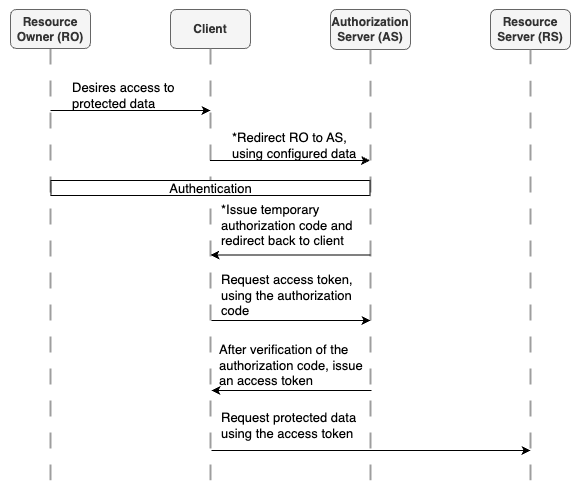
\includegraphics[width=0.75\textwidth]{pic/authorization_code_grant.png}
	\unitlength=0.75mm
	\special{em:linewidth 0.4pt}
	\linethickness{0.4pt}
	\caption{Authorization Code Grant without any extensions}
	\label{fig:auth_code_grant}
\end{figure}

\subsubsection{Implicit Grant}
The Implicit Grant was introduced at a time when there were no mechanisms like Cross-Origin resource sharing implemented in browsers, to share content from different domains. It is a predecessor of the authorization code flow and works similarly with the difference of leaving out the exchanging of the
authorization code step as visualized in figure \ref{fig:implicit_grant}. Instead, the access token is sent via the front
channel directly from the authorization server to the client. This leaves open more attack vectors for example by utilizing the browser history or by
simplifying access token injection \cite{lodderstedt2020oauth}. The Implicit
Grant is officially deprecated, but still has its relevance, as it is still
offered by 37\% of common identity providers \cite{philippaerts2022oauch}.

\begin{figure}[ht]
	\sffamily\footnotesize
	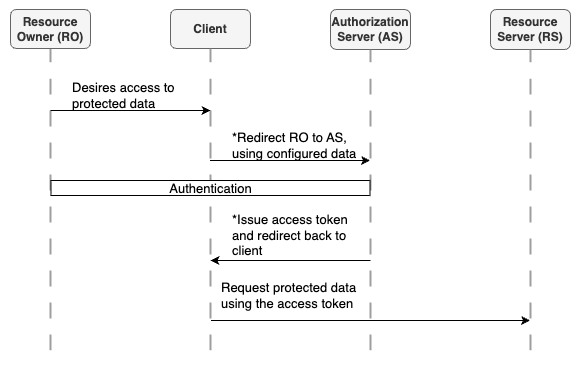
\includegraphics[width=0.75\textwidth]{pic/implicit_grant.png}
	\unitlength=0.75mm
	\special{em:linewidth 0.4pt}
	\linethickness{0.4pt}
	\caption{Implicit Grant}
	\label{fig:implicit_grant}
\end{figure}

\subsubsection{Resource Owner Password Credentials Grant}
This grant type is special in the way that the client is providing its
authentication credentials for the authorization provider to the resource
provider instead, as illustrated in figure \ref{fig:resource_owner_password_credentials_grant}. The resource provider than uses the credentials to retrieve
authorization from the authorization provider. This grant type is only feasible
for the scenario, that the resource provider is trusted completely \cite[Sec.
4.3.]{hardt2012rfc}.

\begin{figure}[ht]
	\sffamily\footnotesize
	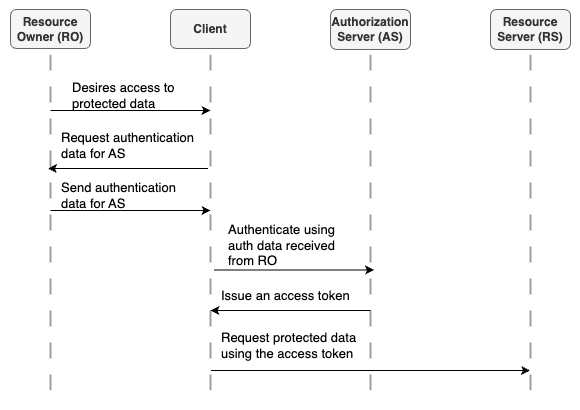
\includegraphics[width=0.75\textwidth]{pic/resource_owner_password_credentials_grant.png}
	\unitlength=0.75mm
	\special{em:linewidth 0.4pt}
	\linethickness{0.4pt}
	\caption{Resource Owner Password Credentials Grant}
	\label{fig:resource_owner_password_credentials_grant}
\end{figure}
	

\subsubsection{Client Credentials Grant}
The client credentials grant must only be used by confidential clients
interacting with each other. This means the clients have the ability to
securely store a secret, which is only accessible by themselves. A common
use-case for this scenario would be machine-to-machine interactions. This grant type is meant for clients to access their own resources as is the case in micro-service architectures. As depicted in figure \ref{fig:client_credentials_grant} the client authenticates at the authorization
server with its client secret and receives an access token, to authenticate at the resource provider. This means that the resource provider does not need to verify client secrets, but instead only needs the capability to verify access tokens. This fact is useful for practical reasons, as a resource provider could reuse the implementation of access tokens for other grant types it is offering.
\cite[Sec. 4.4.]{hardt2012rfc}

\begin{figure}[ht]
	\sffamily\footnotesize
	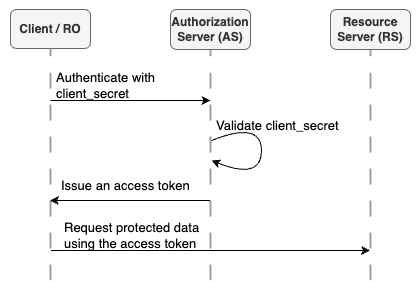
\includegraphics[width=0.6\textwidth]{pic/client_credentials_grant.png}
	\unitlength=0.75mm
	\special{em:linewidth 0.4pt}
	\linethickness{0.4pt}
	\caption{Client Credentials Grant}
	\label{fig:client_credentials_grant}
\end{figure}

\subsubsection{Device Authorization Grant}
Introduced in RFC8628 the device authorization grant is meant to be used for
devices, that lack a user agent like a web browser or do not offer a convenient
way of entering text \cite{denniss2019oauth}. In this grant type the client is
not mainly interacting through a user agent like a web browser anymore, but instead is using a device authorization endpoint at authorization provider directly to initiate an authorization request. The client, then instructs the user to open a webpage on a secondary device to complete the authorization process using a displayed code for verification of the session. This OAuth flow still requires the involved devices to use HTTP for communication, which in general is not a feasible solution for many IoT-devices. A solution for the popular IoT-protocol CoAP is proposed by Chung et al. 

\begin{figure}[ht]
	\sffamily\footnotesize
	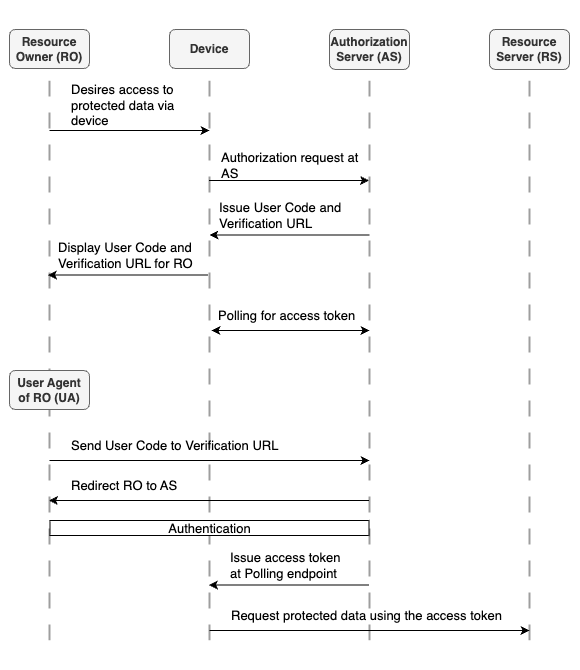
\includegraphics[width=0.75\textwidth]{pic/device_authorization_grant.png}
	\unitlength=0.75mm
	\special{em:linewidth 0.4pt}
	\linethickness{0.4pt}
	\caption{Device Authorization Grant}
	\label{fig:device_authorization_grant}
\end{figure}

\subsubsection{Other grant types}
There are several more grant types, which got introduced to the OAuth standard
over time, which are listed below, but are out of scope for this work: 

\begin{itemize}
	\item Refresh Token Grant
	\item JWT Bearer Grant
	\item UMA Grant
	\item SAML 2.0 Bearer Grant
	\item Token Exchange Grant
\end{itemize}

\subsection{Open ID Connect}
Open ID Connect (OIDC) is a layer on top of OAuth 2.0, introduced in 2014 by a combination of researchers and companies like Google, Microsoft and Salesforce, which form the OpenID group. The main focus of Open ID Connect is authentication, which means identifying a user but not authorizing the user. OIDC flows use a particular OAuth scope, which is called "openid", an extra token, the "ID token", which is a JWT token containing the identifying information about the user, which are called claims. The claims can be used to retrieve more information about the user at the OpenID provider, or the information can be directly part of the initial ID token, so OpenID adds the authentication to the already provided Authorization capability of OAuth. For OIDC, the same grants are used as for OAuth, but in the context of OIDC, they are often referred to as flows \cite{li2016analysing} \cite{sakimura2014openid}.

\subsection{The Future: OAuth 2.1}
OAuth 2.1 will be the next version of OAuth. There is currently one draft available at the IETF \cite{ietf-oauth-v2-1-09}. The main intent of this draft is to consolidate the various extensions to OAuth introduced in the last years. It simplifies the core document for OAuth 2.0 and omits outdated features because of new browser capabilities, which came over the last years and allow for more secure interactions. Below is a list of significant changes:
\begin{itemize}
	\item The Implicit Grant gets omitted
	\item The Resource Owner Password Credentials Grant gets omitted
	\item PKCE is required for the Authorization Code Grant
	\item Redirect URIs must be compared with exact string matching, so pattern matching is completely disallowed
	\item Access tokens must not be transported in a Request-URI in any case (which also makes the Implicit Grant impossible
\end{itemize}

In conclusion, the draft for OAuth 2.1 picks valuable features of existing standards for OAuth to require them and omits outdated features, intending, on the one hand, to simplify the OAuth landscape and, on the other hand, get rid of insecure features of the past.

\section{Intrusion Detection System}
\todo{Fundamental Knowledge: Make clearer that the long definitions use one source}
An intrusion is any malicious behavior with the intention to damage or take control of an information system. All primary protection goals of information security, like confidentiality, integrity and availability, can be the target of an intrusion. A method to harden systems against intrusions is using intrusion detection systems (IDS), which monitor all traffic, events or actions of a system to detect when malicious actions are executed so the system's owner, the administrator or the system itself can take immediate action on intrusion attempts. If the intrusion detection system takes action to prevent intrusions, it is called an \emph{Intrusion Detection and Prevention System (IDPS)} \cite{scarfone2010intrusion}. There are several taxonomies for intrusion detection system types. For example, \cite{Liao2013IntrusionDS} categorized IDS into five categories: Statistics-based, Pattern-based, Rule-based, State-based, and Heuristic-based, referring to the methodology of detection the IDS is using. \cite{khraisat2019survey} build on top of that approach to further specify an overall taxonomy for IDS, which is used in this work to define Intrusion Detection Systems. 

\subsection{Distinction by input data}
Generally, when categorizing Intrusion Detection Systems by environment or input data, there are two types to distinguish them. 
\emph{Host-based Intrusion Detection Systems (HIDS)} and \emph{Network-based Intrusion Detection Systems (NIDS)}.
\subsubsection{Host-based Intrusion Detection System}
HIDS monitor all data concerning a host system, like operating system events, host firewall logs or application-specific logs. They can detect specific attacks on the system level without using network logs.
\subsubsection{Network Intrusion Detection System (NIDS)}
NIDS monitor network traffic, which is acquired by packet capture tools and other network data sources. One challenge of Network Intrusion Detection Systems is often the large amount of data that needs to be analyzed in high-bandwidth networks, which demands high computing capabilities.

\subsection{Distinction by detection characteristic}
When distinguishing types of intrusion detection systems by the way they operate, there are two categories: Signature-based (SIDS) and Anomaly-based (AIDS).

\subsubsection{Signature-based Intrusion Detection System}
Signature-based IDS utilize databases of fingerprints of already known attacks. These databases are called knowledge databases. A fingerprint could be, for example, a hash value of an executable malware file. A HIDS could compare any file an operating system executes against the knowledge database to detect the specific malware. The same concept also works for NIDS, e.g., when scanning mail attachments transferred via SMTP. The main advantage of SIDS is that they rarely produce false positive alerts when identifying intrusions. Their downside is that they cannot detect unknown attacks.

\subsubsection{Anomaly-based Intrusion Detection System}
The core concept for Anomaly-based IDS is to differentiate between usual and unusual behaviour. Unusual behaviour is identified as an intrusion. There is a variety of techniques that AIDS can use to achieve the goal of differentiating typical and malicious behaviour. One possibility is creating a statistical model over the data and filtering out events with a low probability. 
Another approach is to use machine learning techniques. Unsupervised learning methods, like clustering, on the one hand, are very similar to the statistical approach because the goal is again to sort out rare occurrences in small clusters. Supervised learning methods, on the other hand, create a model of usual behaviour in a training phase with labelled data to test any new input of unknown data if it is classified as malicious. 
An additional way for Anomaly-based IDS is the knowledge-based method. With this method, knowledge is applied to the detection in the form of rules to identify any behaviour that breaks those rules as an intrusion. These rules can stem from knowledge about a network protocol or any other system behaviour.

\subsection{zeek IDS}
\todo{Fundemental Knowledge: Write zeek section}

\section{Algorithms}
\todo{Describe the algorithms used in the experiments}

\chapter{Related Work}
\label{chap:related_work}
\todo{Write Introduction to Related Work chapter}
\section{Security Analysis of OAuth}
\cite{fett2016comprehensive}
\todo{Realted Work: Describe Security Analysis of OAuth}

\section{Machine Learning approach to detect OAuth vulnerabilities}
\cite{munonye2022machine}
\todo{Related Work: Describe approach to detect OAuth vulnerabilities}
\section{Another One}
\todo{Related Work: Decide on which 1-2 more articles to mention here aswell}


\chapter{OAuth Security}
\todo{Write Introduction to OAuth Security chapter}
\section{Threats and Vulnerabilities}

\subsection{Insufficient Redirect URI Validation \cite{lodderstedt2020oauth} \cite{wang2019make}}
Authorization Servers need to whitelist redirection URLs in order to make sure,
that an attacker cannot craft a hyperlink, which leads to the victim initiating
an OAuth flow and sending the authorization code or token to an
attacker-controlled domain. Some authorization servers may allow the usage of
patterns in order to allow several domains at once. As well as the absence of
any sort of whitelist mechanism even a pattern-matching functionality could
lead to security problems. Among the possibility that a user is entering
patterns that are too broad and allow the usage of unintended redirect URLs,
the attack surface includes issues with the URL parsing implemented by the
authorization server as shown by Wang et al. \cite{wang2019make}. They
presented several techniques to trick the parser into accepting unintended
domain names, like using squared brackets for IPv6 parsing or the \emph{Evil
Slash Trick}, where the parser does not treat a forward slash as a path
separator, while modern browsers do. Depending on the OAuth grant type in use
this vulnerability leads to different possibilities to exploit it.


\subsubsection{Authorization Code Flow}
\begin{itemize}

    \item The attacker uses techniques like phishing to make its victim open an
        attacker-controlled webpage, which initiates an OAuth flow with the
        vulnerable authorization server.
	
    \item The request is crafted with a valid client ID (which is public
        information), ``code'' as response type and a malicious redirect URI,
        which leads to an attacker-controlled server again.
	
    \item If the user logs in at the authorization server, the authorization
        code now gets transmitted to the attacker's webpage, via the redirect
        URI.
	
    \item The attacker page can now use the received authorization code, to
        retrieve a token 

\end{itemize}

\subsubsection{Implicit Flow}
\todo{Maybe write down open redirection with the implicit flow here regarding redirect\_uri check circumvention}


\subsection{Credential Leakage via Referer Headers}
The Referer HTTP header is a potential attack surface. It can be utilized by a
malicious actor to capture query parameters, which are sent via the front
channel, like the state and the authorization code. The authorization code may
be used to redeem an access token before the victim retrieves it and the state
parameter oftentimes includes a CSRF token, which could potentially open up
vulnerabilities in other parts of the application as explained by Fett et al
\cite{fett2016comprehensive}.

\subsubsection{OAuth Client}
If a client renders third-party content, like advertisements in iframes or
images, before redeeming the authorization code for an access token an
attacker, who places these advertisements or images can capture the code via
the referer header and redeem it for an access token.

\subsubsection{Authorization Server}
At the authorization server, the state parameter could be leaked via the
Referer header, when 3rd party images or advertisements are being rendered on
the page. This may be an issue when the state contains a CSRF token as
explained by Fett at al \cite{fett2016comprehensive}.


\subsection{Credential Leakage via History Logs}
OAuth potentially transports sensitive data via the request-URI, like the access token, as is the case when the implicit grant is used or if other grant types optionally allow the transportation of access tokens or authorization codes via URI parameters. Therefore, a person accessing the user's browser can extract this sensitive data and try to replay it. The same threat is present when a logging server is present, for example, in a corporate network \cite{lodderstedt2020oauth}. Research about browser history security focuses mainly on accessing information about the victim's history by comparing cache timings if a page was visited \cite{bansalcache}. This type of threat is irrelevant in the OAuth context because an attacker would need to guess the access token, which the attacker could endeavor outside the browser history as well. However, recent studies on the security of browser extensions show that malicious browser extensions could access the browser history, or data could be leaked by utilizing vulnerable browser extensions \cite{eriksson2022}.

\subsubsection{Countermeasures}
- Authorization Code
- Access Token


\subsection{Mix-Up Attack}
In this attack, at least two authorization providers are involved. The target AP and the attacker AP. The OAuth standard allows the resource provider to interact with multiple authorization providers, one of which could be malicious, so the security for such interactions must also be provided. The attack is feasible for the implicit and authorization code grants and works similarly for both. Another precondition is that the resource owner registers the same redirect URI at both authorization providers, which is typical for Open ID Connect dynamic client registration \cite{hosseyni2023formal}. With these preconditions present, the attacker now waits until the target initializes an OAuth flow with the attacker AP. The attacker then intercepts the initialization request and exchanges the target AP with its attacker AP. When the target client gets redirected to the attacker AP, the target gets immediately redirected back to the target AP for authentication. At the same time, the client ID in the query parameters of the redirection URL gets replaced with the one registered at the target AP. Suppose the target user authenticates because it did not detect that it intended to authenticate at another AP. In that case, an authorization code gets issued to the client when the authorization code grant used. The client then proceeds to try to redeem an access token at the attacker AP, as the client still thinks that it initiated an OAuth flow with the attacker AP. The attacker can now use the received authorization code to redeem an access token at the target AP. \cite{fett2016comprehensive}

\subsection{Authorization Code Injection \cite{philippaerts2022oauch}} 
The precondition for an authorization code injection is that an attacker has
successfully stolen an authorization code. This can be accomplished in various
ways for example by tricking the user into installing a malicious browser
extension, using other vulnerabilities in a web app like open redirections, or
abusing proxy auto-configuration files \cite*{philippaerts2022oauch}.

In the case, that the client is using the authorization code flow the attacker
can use the stolen authorization code to fetch an access token before the
client does.

\subsubsection{Countermeasures}
There are several ways to mitigate the risk of authorization code injection.
For example, if an authorization code got used twice in the case it got stolen
and the attacker, as well as the client, tried to redeem a token, every token
that was redeemed with this authorization code should get invalidated. Another
method is the usage of PKCE to make sure the OAuth flow is only used, between
the two legitimate parties.



\subsection{Access Token Injection}
This kind of attack describes the process of an attacker using a stolen access
token in a legitimate authentication flow, to impersonate the client. If the
implicit flow is available, the attacker can now start a new flow and simply
replace the access token in the authorization servers' response. This will
circumvent any CSRF protection, as there is no difference to a non-compromised
flow. \cite{lodderstedt2020oauth}


\subsection{Cross Site Request Forgery}
This type of attack, often referred to by its abbreviation ``CSRF"", is about
the attacker executing a request in the name of the user, by tricking the user
into executing requests for the attacker including all required authentication,
or authorization information. The default OAuth protocol does not include
protection mechanisms against this type of attack. 

\subsection{PKCE Downgrade Attacks}
If an authorization server is not implemented to require PKCE for all its
flows, it is susceptible to being vulnerable to PKCE downgrade attacks
\cite{philippaerts2022oauch}. Even if it is documented otherwise, attackers
might try to omit PKCE parameters, as the current OAuth 2.0 standard does not
require the usage of the PKCE extension \cite{hardt2012rfc}. 


\subsection{Access Token Leakage at the Ressource Server}
In the scenario that clients can dynamically connect to resource servers at runtime, as is the case in mail or banking applications, an attacker could create a malicious resource server and trick the user into sending valid access tokens for the target data to the malicious resource server. It could also be the case that the client application is misconfigured to send access tokens to a dynamically created resource server. Another vector for Access token leakage at the resource server is when the server itself gets compromised, so the attacker receives access tokens by analysing connections to the server itself \cite{lodderstedt2020oauth}.

\subsection{307 Redirect}
The OAuth standard does not specify which type of HTTP redirect should be implemented to redirect the user back to the client after the authentication at the authorization provider is successful. As the HTTP 307 redirect reuses the header and the body of the original request \cite{fielding1999rfc2616}, a malicious client could extract the username and password of the initial form submission action because it receives this data as part of the redirection \cite{fett2016comprehensive}.

\subsection{Client Impersonating Resource Owner}
In the scenario that an authorization server allows for multiple grant types, including the client credentials grant and another typical grant like the authorization code grant, the threat of a malicious client impersonating a resource owner can be present in certain implementations. One example is when the authorization server allows for dynamic registration of clients, with the possibility of setting a client ID. A client could set its ID to the value of an identifying value of a resource owner. To build the example further, Open ID Connect uses a token's subject property to identify a user \cite{sakimura2014openid}. A client could use the subject value as its client ID. Improper implementations of resource servers, which do not distinguish between token types by grant type, could mistake an access token issued to a resource owner with a token issued to a client, which allows the malicious client to access the protected data of the resource owner \cite{lodderstedt2020oauth}.


\subsection{Authorization Server Redirecting to Phishing Site}
\label{sub:authorization_server_redirecting_to_phishing_site}
When the authorization server allows dynamic client registration, an attacker could create a valid client to which the authorization server could redirect. The attacker then crafts a malicious authorization request that will always fail by appending an invalid \emph{scope} value and then will redirect to the phishing site. An example of such a malicious authorization request is depicted in Figure \ref{fig:phishing_requests}. As the authorization attempt using this crafted URL is always invalid because of the \emph{scope}, the victim immediately gets redirected back to the site given by the \emph{redirect\_uri} parameter, which legally got enlisted through dynamic client registration. This site could be a copy of the valid login page to trick the user into entering its credentials. This way of phishing is very subtle as the domain of the phishing link is valid and known by the victim. The victim would need to identify that the \emph{redirect\_uri} query parameter is invalid and realize that it gets redirected to this URL after clicking on the link with the valid domain \cite{lodderstedt2020oauth}.


\begin{figure}[ht]
	\sffamily\footnotesize
	\url{https://valid-site.com/authorize?scope=invalid&redirect_uri=https://phishing-site.com/login&client_id=client_id_of_malicious_client}
	\special{em:linewidth 0.4pt}
	\linethickness{0.4pt}
	\caption{Phishing request}
	\label{fig:phishing_requests}
\end{figure}

\subsection{Unvalidated Redirects and Forwards}
This type of vulnerability, known as \emph{Unvalidated Redirects and Forwards} (URF) as well as \emph{Open Redirect}, exists when a web application exposes redirection or forward capabilities to untrusted user input, for example, through query parameters. An attacker could generally utilize URF vulnerabilities to craft phishing links that are masked with valid, trustworthy domains \cite{wang2015urfds}. Especially in connection with OAuth, an attacker using an existing URF vulnerability in a client can potentially circumvent whitelists for redirection URIs, by masking the redirect to a malicious client with a valid client exposing an open redirect in the query parameter \cite{lodderstedt2020oauth}. Section \ref{sub:authorization_server_redirecting_to_phishing_site} describes a different attack aimed at masking a phishing attack utilizing a mechanism specific to OAuth that is similar to an open redirection at the authorization server and therefore a threat, which is introduced by the implementation of OAuth itself.

\subsection{Clickjacking}
As authorization providers authorize applications to access confidential data, they are susceptible to being targeted by clickjacking attacks. Clickjacking attacks trick users into performing clicks on elements on a web page the users did not intend to interact with, e.g., by overlaying invisible iframes. In the case of OAuth, an attacker could create a malicious application and register it at the authorization provider of the target. The attacker also prepares a webpage that tricks the user into clicking on an invisible iframe of the authorization provider. The iframe could contain the grant access step of allowing the malicious application to access the user's confidential data. If the user has an active session at the authorization provider, a single click is enough to fulfill this action \cite{gibbons2014security}. 


\section{Countermeasures}
\subsection{PKCE system}
As an extension to OAuth defined by RFC 7636, ```Proof Key for Code Exchange''
is a technique to mitigate Authorization Code Injection misuse or CSRF attacks
\cite{bradley2015rfc}. Specifically, it extends the authorization code flow 
\todo{OAuth Security: Finish section about PKCE}

\subsection{Refresh Token Protection}
\todo{OAuth Security: Write about Refresh Token Protection}

\subsection{Misuse of Stolen Access Tokens as Countermeasure}
\todo{OAuth Security: Write about Misuse of Stolen Access Tokens}

\section{OAuth Threats by Mitigation Responsibility}

\begin{figure}[!htb]
	\sffamily\footnotesize
	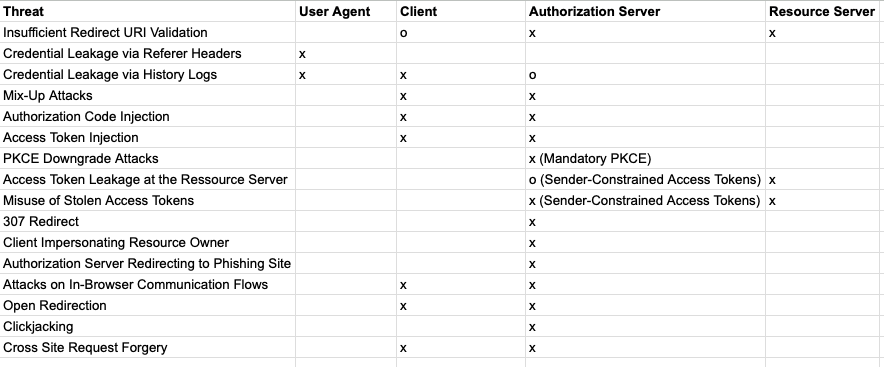
\includegraphics[width=1\textwidth]{pic/threats.png}
	\unitlength=0.75mm
	\special{em:linewidth 0.4pt}
	\linethickness{0.4pt}
	\caption{Draft Table (Make LaTeX table, when table is finalized)}
	\label{fig:threats_by_mitigation}
\end{figure}

\todo{Maybe add countermeasures to table}
\todo{Make LaTeX table with finished overview}


\chapter{Intrusion Detection Approach}
\todo{Maybe integrate this chapter into \ref{chap:exp}}

\section{k-nearest neighbor}

\section{k-means clustering}

\section{Rule-based techniques}
\subsection{Count auth code usages}
\subsection{Seperate flows and check completion}


\chapter{Experimental Analysis}
\label{chap:exp}
This chapter examines the capabilities of the intrusion detection techniques and algorithms presented in chapter \ref{chap:exp}.

Initially, section \ref{sec:exp_setup} describes the experimental environment for dataset generation and analysis. This section is subdivided into three parts to describe the multi-step process that was implemented to generate and analyze datasets for the experiments.

\section{Environment Setup}
\label{sec:exp_setup}
An essential piece for this research and its experiments is the dataset for testing intrusion detection methods. At the time of this writing, a dataset of network logs with specific attacks on OAuth does not exist. Hence, the first part of the experimental setup is the dataset generation. 

\subsection{OAuth flow execution and Logging}
For this first part, an OAuth environment was implemented, which consists of several subsystems that are needed to execute the OAuth protocol flow. This experimental setup is illustrated in Figure X. \todo{Experimental Analysis: Create figure of experiment environment} It consists of two independent networks. The first network contains the authorization provider and a logging service, and the second network contains the OAuth client service and a logging service. The loggers produce .pcap-files of all activity in their network using "tcpdump". 

The OAuth authorization framework is practice-oriented. Therefore, the network logs are divided between the auth provider and the client, as in practice, mostly two different parties run these services. The auth provider implements four OAuth grants, which are among the most essential grants, namely "Implicit Grant", "Authorization Code Grant", "Client Credentials Grant", and "Password Grant". It also implements extensions like the "Refresh Token Grant" and the "PKCE"-extension. In addition to the Authorization capabilities, the auth provider service also offers a protected resource in the form of an API, which is only accessible by authorized clients. The protected endpoint is '/api/me' and returns the username of the authenticated and authorized user.

The client is a simple static webpage that handles the authorization code flow. It can be used to generate traffic manually, but its primary purpose is to handle redirections as part of the different flows. It is written in HTML, CSS, and Javascript to utilize the Fetch API and the Browser Storage API.

The following service is the attacker server implemented in Python using the "http.server" library, which serves the purpose of a callback handler for attacks that redirect the victim's OAuth flows to the attacker. It also completes OAuth flows with stolen authorization codes or access tokens and generates traffic at the auth provider like this.

\subsection{Fuzzing}
The above-described services create a complete environment for executing valid OAuth flows and attacks on OAuth. A generator service was implemented in Python to utilize this whole setup to produce network logs. The generator uses fuzzing to generate network traffic, including attacks randomly, which then gets logged by the logger services attached to the networks of the auth provider and client. The generator also logs whenever an attack is executed in its process output.

\subsection{Analysis}
The last piece of the experimental setup is the intrusion detection mechanism. This part is again a multi-step process. In the beginning, the network logs of the logger services are statically analyzed by the "zeek" IDS using the "--readfile" option of zeek. Zeek then produces so-called "zeek-logs". In order to process the zeek-logs, the "zat" library is used to load the data into Python "pandas" data frames. The reason for this is that "pandas" is a popular Python data analysis library, which already implements several valuable functions, like clustering or model-based algorithms.



\chapter{Conclusion}


% =============================Literaturverzeichnis=============================
\begin{raggedright}         % Schaltet Blocksatz ab, erzeugt ein stimmigeres
                            %  Schriftbild im Literaturverzeichnis.
  \printbibliography        % Falls Biblatex verwendet wird.
  \label{sec:literaturverzeichnis}
\end{raggedright}


% ===================================Anhang=====================================
\appendix
\setcounter{figure}{0}
\renewcommand\thetable{A.\arabic{figure}}
\setcounter{table}{0}
\renewcommand\thetable{A.\arabic{table}}
% ===========================Selbstständigkeitserklärung======================
\chapter*{Eidesstattliche Versicherung} % war: Selbständigkeitserklärung
\vspace{1cm}

\todo[noline]{Bitte verwenden Sie hier in jedem Fall die offizielle von der Prüfungsbehörde vorgegebene Formulierung der Selbständigkeitserklärung.}
%
Hiermit versichere ich an Eides statt, dass ich die vorliegende Arbeit
selbstständig verfasst und keine anderen als die angegebenen Hilfsmittel –
insbesondere keine im Quellenverzeichnis nicht benannten Internet-Quellen –
benutzt habe. Alle Stellen, die wörtlich oder sinngemäß aus Veröffentlichungen
entnommen wurden, sind als solche kenntlich gemacht. Ich versichere weiterhin,
dass ich die Arbeit vorher nicht in einem anderen Prüfungsverfahren eingereicht
habe und die eingereichte schriftliche Fassung der auf dem elektronischen
Speichermedium entspricht.

Ggf. streichen: Ich bin damit einverstanden, dass meine Abschlussarbeit in den
Bestand der Fachbereichsbibliothek eingestellt wird.

\makeatletter
Hamburg, den {\@date}
\makeatother

\vspace{2cm}
\rule{6cm}{0.25pt}\\
\makeatletter
{\@author} \par
\makeatother




% ================================Literaturliste-Muster==============================
\newpage
\thispagestyle{empty}
\label{sec:literaturliste}
\par\textbf{\textsf{Thema:}} Privacy Enhancing Technologies zum Schutz von Kommunikationsbeziehungen
\par\textbf{\textsf{Bearbeiter:}} Eva Musterfrau, Heinz Mustermann
\par\textbf{\textsf{Datum:}} \today
\bigskip
% ====> Delete me
\begin{tikzpicture}[overlay]
    \node[draw, blue, font=\sffamily\Large, xshift=70mm, yshift=0mm, rounded corners=1mm]{Muster der Literaturliste};
\end{tikzpicture}
% <==== /Delete me
\par\textbf{\Large\textsf{Literaturliste}}

% ================================Todo list==============================
\listoftodos
% \todototoc

\end{document}
